\documentclass[12pt,a4paper]{scrartcl}
\usepackage{ifpdf}
%\usepackage[utf8]{inputenc}
\usepackage[ngerman]{babel}
\usepackage{amsmath}
\usepackage{amssymb}
\usepackage{fancyhdr}
\usepackage{listings}
\usepackage{color}
\usepackage{pdfpages}
\pagestyle{fancy}
\fancyhead{}
\fancyfoot{}
\fancyhead[LO,LE]{Johannes Hedtrich, Christopher Hlubek}
\fancyhead[RO,RE]{Serie 02}
\fancyfoot[CO,CE]{\thepage}

\title{Serie 02}
\author{Johannes Hedtrich, Christopher Hlubek}
\date{\today}
\begin{document}

\section*{2.3 Dualitätsprinzip}

Die Menge $NNF_{AL}$ ist induktiv definiert durch:
\begin{enumerate}
  \item Basismenge: Die Basiselemente sind 0, 1 $X_i$, und $\neg X_i$ für $i \in \mathbb{B}$
  \item I\lstset{language=c++}nduktionsregeln: Sind $\varphi, \psi \in NNF_{AL}$, so sind $(\varphi \vee \psi) in NNF_{AL}$ und $(\varphi \wedge \psi) \in NNF_{AL}$
\end{enumerate}

Zu jeder Formel $\varphi \in NNF_{AL}$ ist die zu ihr duala Formel $\overline{\varphi}$ induktiv definiert durch:
\begin{enumerate}
  \item Basiszuordnung: $\overline{0} = 1$, $\overline{1} = 0$, $\overline{X_i} = \neg X_i$, $\overline{\neg X_i} = X_i$
  \item Induktionsregeln: Für alle $\varphi, \psi \in NNF_{AL}: \overline{\varphi \wedge \psi} = \overline{\varphi} \vee \overline{\psi}, \overline{\varphi \vee \psi} = \overline{\varphi} \wedge \overline{\psi}$.
\end{enumerate}

\textbf{Behauptung:} Für jedes $\varphi \in NNF_{AL}$ gilt: $\neg \varphi \equiv \overline{\varphi}$

\textbf{Beweis:}\\
Induktionsanfang:\\
$\neg 0 = 1 = \overline{0}$\\
$\neg 1 = 0 = \overline{1}$\\
$\neg X_i = \overline{X_i}$\\
$X_i = \neg \neg X_i = \overline{\neg X_i}$\\

Induktionsschluss:\\
$\neg (\varphi \vee \psi) \equiv \neg \varphi \wedge \neg \psi \equiv \overline{\varphi} \wedge \overline{\psi} \equiv \overline{\varphi \vee \psi}$\\
$\neg (\varphi \wedge \psi) \equiv \neg \varphi \vee \neg \psi \equiv \overline{\varphi} \vee \overline{\psi} \equiv \overline{\varphi \wedge \psi}$\\

\section*{2.4 formula to string}
siehe Anhang.
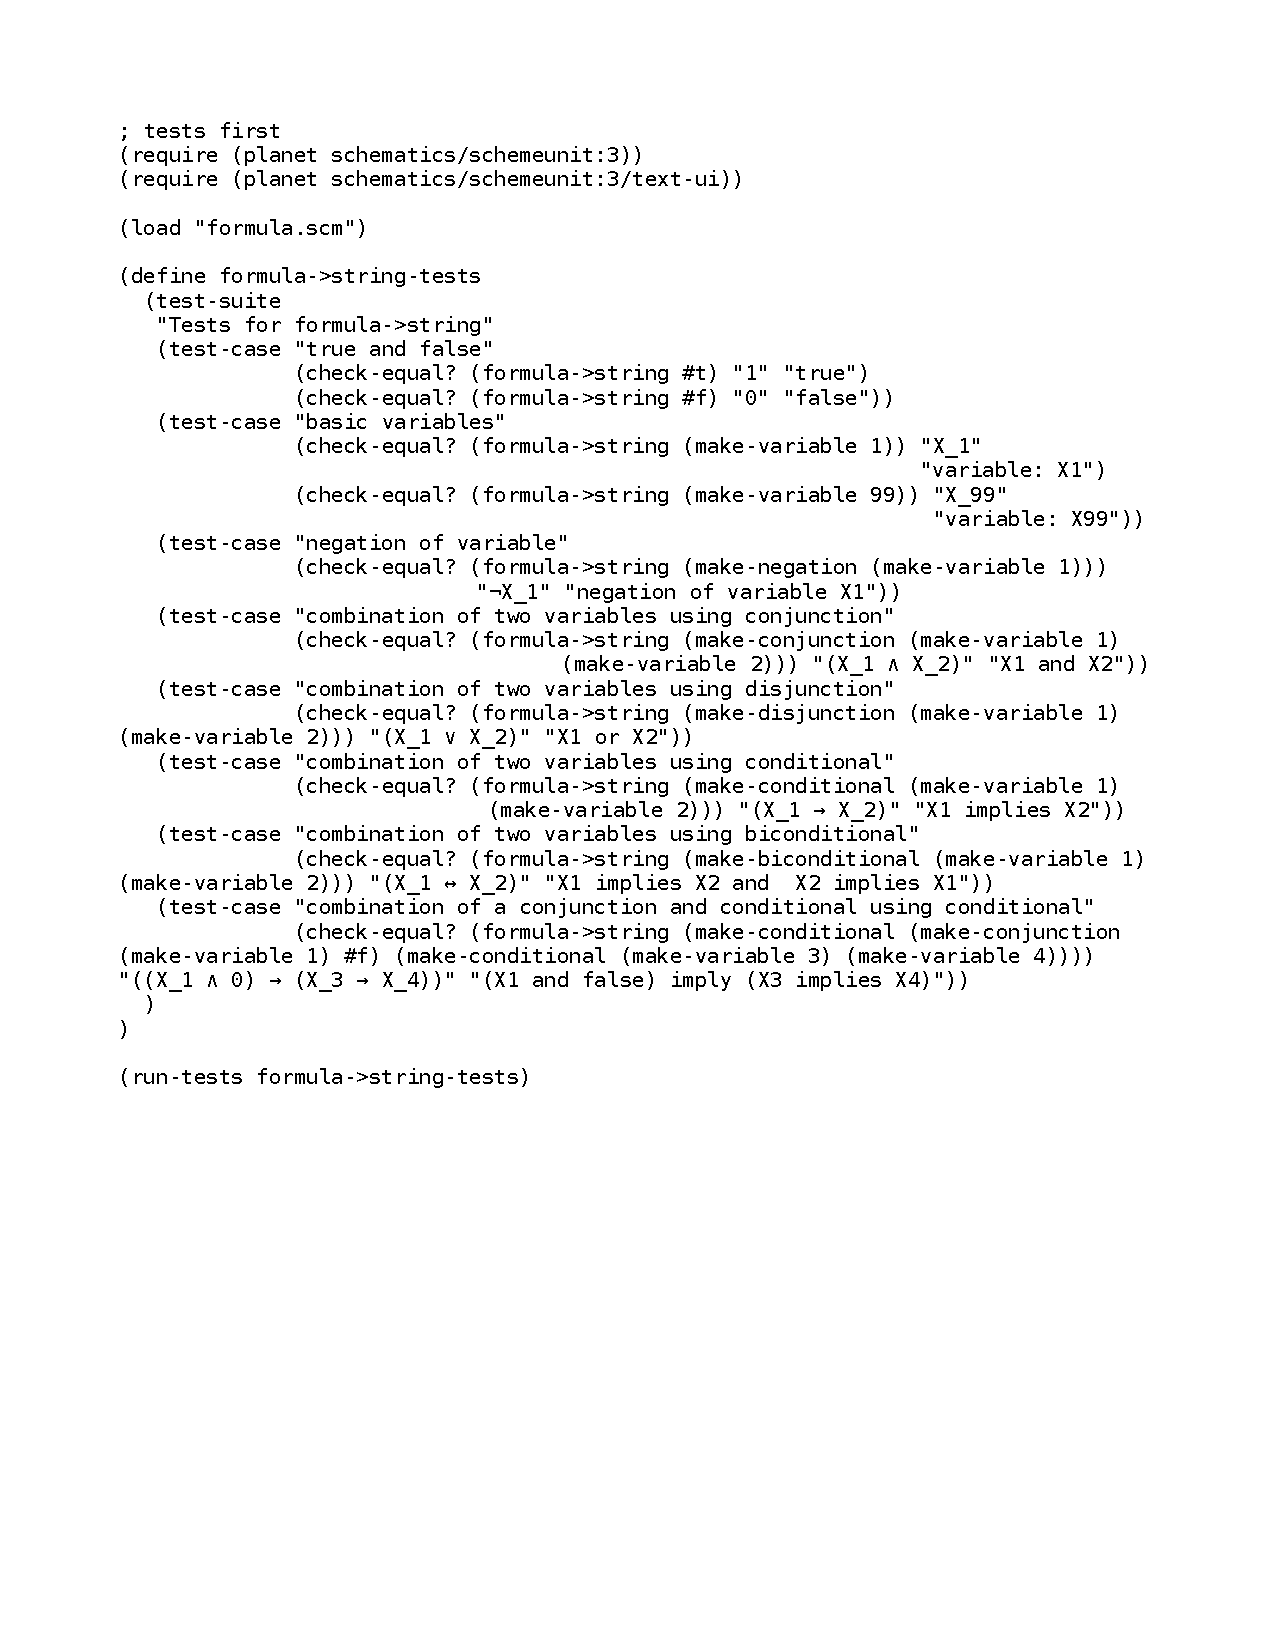
\includepdf[pages=-]{code.pdf}
\end{document}

